\begin{document}
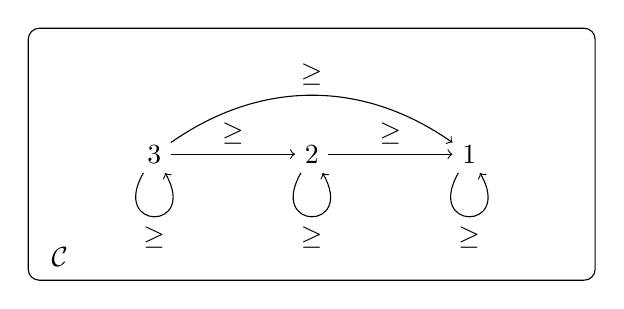
\begin{tikzpicture}
  \draw[rounded corners] (-1.6,-1.6) rectangle (5.6,1.6);
  \node at (-1.2,-1.3) {$\mathcal{C}$};
  \node (3) at (0,0) {$3$};
  \node (2) at (2,0) {$2$};
  \node (1) at (4,0) {$1$};
  \draw[->] (3) -- node[above] {$\geq$} (2);
  \draw[->] (2) -- node[above] {$\geq$} (1);
  \draw[->] (3) to[bend left=35] node[above] {$\geq$} (1);
  \draw[->] (3) to[out=-120,in=-60,looseness=8] node[below] {$\geq$} (3);
  \draw[->] (2) to[out=-120,in=-60,looseness=8] node[below] {$\geq$} (2);
  \draw[->] (1) to[out=-120,in=-60,looseness=8] node[below] {$\geq$} (1);
\end{tikzpicture}
\end{document}
